\documentclass[11pt]{article}

% basic packages
\usepackage[margin=2cm]{geometry}
\usepackage[pdftex]{graphicx}
\usepackage{amsmath,amssymb,amsthm}
\usepackage{custom}

% page formatting
\usepackage{fancyhdr}
\pagestyle{fancy}

\renewcommand{\sectionmark}[1]{\markright{\textsf{\arabic{section}. #1}}}
\renewcommand{\subsectionmark}[1]{}
\lhead{\textbf{\thepage} \ \ \nouppercase{\rightmark}}
\chead{}
\rhead{}
\lfoot{}
\cfoot{}
\rfoot{}
\setlength{\headheight}{14pt}

\linespread{1.03} % give a little extra room
\setlength{\parindent}{0.2in} % reduce paragraph indent a bit
\setcounter{secnumdepth}{2} % no numbered subsubsections
\setcounter{tocdepth}{2} % no subsubsections in ToC

\begin{document}

% make title page
\thispagestyle{empty}
\bigskip \
\vspace{0.1cm}

\begin{center}
{\fontsize{36}{36} \selectfont \bf \sffamily Probability Notes}
\vskip 24pt
{\fontsize{18}{18} \selectfont \rmfamily Conor Redington} 
\vskip 24pt
\end{center}

% make table of contents
\newpage
\microtoc
\newpage

% main content
\hypertarget{probability}{%
\section{Probability}\label{probability}}

\_following along course in MIT opencourseware\_\_ \emph{The goal is to
have a resource that lays out my fundamental understanding of
probability} My thoughts on probability\_ are scattered.

https://ocw.mit.edu/courses/6-041sc-probabilistic-systems-analysis-and-applied-probability-fall-2013/
*
https://ocw.mit.edu/courses/res-6-012-introduction-to-probability-spring-2018/

Sample space is just a set of outcomes of experiment, which can be
discrete, finite, infinite etc.

This is also similar to leaves in a tree, or the garden of forking data.
Just ways of representing the set of possible outcomes.

Events are subsets of the sample space. This is because you can't assign
a definite probability to an continuous set taking on a particular
value.j

\hypertarget{axioms}{%
\section{Axioms}\label{axioms}}

There are a basic set of axioms (3) that can be used to derive all the
useful properties of the probability mathematical model.

\hypertarget{discrete-uniform-law}{%
\subsubsection{Discrete Uniform Law}\label{discrete-uniform-law}}

\begin{itemize}
\tightlist
\item
  Assume \(\omega\) consists of \(n\) equally likely elements.
\item
  Set A consists of \(k\) elements. The \(P(A) = k\frac{1}{n}\).
\end{itemize}

\hypertarget{probability-calculation-steps}{%
\subsection{Probability calculation
steps:}\label{probability-calculation-steps}}

\begin{itemize}
\tightlist
\item
  Specify the sample space. Can draw it out. Tree diagrams, for example
  are just a representation of the sample space.
\item
  Specify the probability law (arbitrary).
\item
  Identify an event of interest.
\item
  Calculate. Use pictures!
\end{itemize}

\href{https://www.youtube.com/watch?v=mUxg3j_h5GM\&list=PLUl4u3cNGP60hI9ATjSFgLZpbNJ7myAg6\&index=9}{Is
area a legitimate probability law for a unit square. Countable
additivity, how our disjoint axiom only applies to countable infinities}

\hypertarget{conditional-probability}{%
\section{Conditional Probability}\label{conditional-probability}}

\begin{itemize}
\item
  useful in reasoning with \textbf{partial information} of the
  occurrence of some event.
\item
  Specification of new probability law (that abides the axioms) to take
  this new information (whatever it is) into account.
\item
  If we know that the outcome of some experiment is in event B get the
  probability that it also lies in A \textbf{using this information}.
\item
  Probability laws are always aiming to quantify beliefs.
\item
  Once B has occurred, it now `becomes' the sample space so it's
  probability of occurring is 1. Almost as if you zoom in on it.
\item
  Need to scale A's original probability when B becomes the sample
  space.
\item
  This is a definition, not a theorem. Motivated by reasoning.
\item
  Sometimes it's useful to just work with the maths of it. Knowing that
  it's a model. So just using the formal rules of sets etc.
\end{itemize}

\hypertarget{mulplication-rule}{%
\subsection{Mulplication Rule}\label{mulplication-rule}}

\begin{figure}
\centering
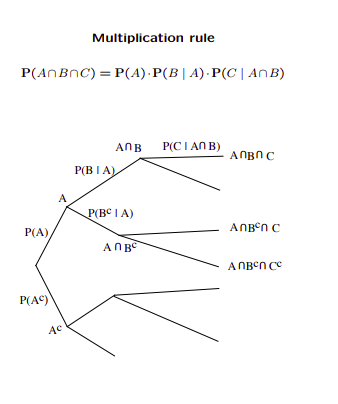
\includegraphics{img/multiplicationrule.png}
\caption{`multiplication rule'}
\end{figure}

\begin{itemize}
\tightlist
\item
  Models involving conditioning normally take on this branching
  approach.
\end{itemize}

\hypertarget{total-probability-theorem}{%
\subsection{Total Probability Theorem}\label{total-probability-theorem}}

\begin{figure}
\centering
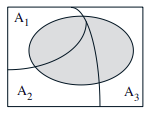
\includegraphics{img/totalprobailitytheorem.png}
\caption{total probability}
\end{figure}

\begin{itemize}
\tightlist
\item
  Visualising event B as happening in a number of `scenarios'.
\item
  The probability that B occurs is then a weighted probability under
  each scenario.
\item
  \(P(B) = P(A_1 \cap B) + ... + P(A_n \cap B)\)
\item
  \(P(B) = P(A_1)P(B|A_1) + ... + P(A_n)P(B|A_1)\).
\item
  When you have a mildly complicated event, that can happen in different
  scenarios.
\end{itemize}

\hypertarget{bayes-rule}{%
\subsection{Bayes Rule}\label{bayes-rule}}

\begin{itemize}
\tightlist
\item
  If we look at a cause effect relationship. Bayes Theorem can be seen
  as giving a belief in the cause (\(A_i\)) of an observed effect B.
\item
  \(P(B|A_i) = \frac{B \cap A_i}{P(A_i)}\)
\item
  We can use the multiplication rule (looking at the tree):
\item
  \(P(A_i|B) = \frac{P(A_i)P(B|A_i))}{P(B)}\).
\item
  Could look at the tree diagram as a causal model. And the left as
  inferring what cause lead to the outcome on the right.
\end{itemize}

\hypertarget{independence}{%
\section{Independence}\label{independence}}

\begin{itemize}
\tightlist
\item
  Two events are independent if the occurrence of one event does not
  change our beliefs about the other.
\item
  Subtly, disjoint and independence are not the same thing! Independence
  is about information.
\end{itemize}

\hypertarget{what-is-the-relationship-between-conditioning-and-independence}{%
\subsection{What is the relationship between conditioning and
independence?}\label{what-is-the-relationship-between-conditioning-and-independence}}

\hypertarget{constructors}{%
\subsection{Constructors}\label{constructors}}

I think the notion of sets is important in that of a constructor. That
we can make a set of anything. Useful when an event could be anything.

\hypertarget{counting}{%
\section{Counting}\label{counting}}

\begin{itemize}
\tightlist
\item
  Useful methods for establishing the sample space.
\end{itemize}

\hypertarget{random-variables}{%
\section{Random Variables}\label{random-variables}}

\begin{itemize}
\tightlist
\item
  Assignments of numbers to every possible outcome.
\item
  \textbf{A function from the sample space \Omega to the real number
  line}.
\item
  We have the random varibale \(X\), which represents the function.
  Tsitsiklis also says you can think of it as a sub routine or process.
  We then have \(x\) the number that X spurts out for an outcome.
\end{itemize}

\hypertarget{pmf}{%
\subsection{PMF}\label{pmf}}

\begin{itemize}
\tightlist
\item
  A probability distribution of X.
\end{itemize}

\hypertarget{how-to-compute-a-pmf}{%
\subsubsection{How to compute a PMF}\label{how-to-compute-a-pmf}}

\begin{itemize}
\tightlist
\item
  Collect all possible outcomes for which X is equal to x.
\item
  Add their probabilities.
\item
  Repeat for all x.
\end{itemize}

\hypertarget{binomial-pmf}{%
\subsection{Binomial PMF}\label{binomial-pmf}}

\begin{itemize}
\tightlist
\item
  Binomial random variable
\item
  Once again, useful to think of trials as coin tosses with some
  probability of H (or T doesn't really matter).
\item
  Binomial random variable is function that takes returns the numerical
  value of the subset of outcomes of n trials that have the `supplied'
  heads.
\item
  We know that each of these outcomes would have the same probability
  (some mixture of heads and not heads) for the n tosses.
\item
  So the pmf for the binomial is (n choose k)\(p^{k}(1-p)^{n-k}\) summed
  over each k value.
\item
  If X is \emph{the number of heads in n tosses} then the pmf for X must
  cover all the k values from 0 to n.
\end{itemize}

\hypertarget{expected-value-of-a-random-variable}{%
\subsection{Expected Value of a Random
Variable}\label{expected-value-of-a-random-variable}}

\begin{itemize}
\tightlist
\item
  Can be interpreted a center of gravity of an object of the kind given
  by the pmf. Mainly useful for symmetric pmf's.
\item
  \[E[X] = \sum_xxp_X(x)\]
\item
  In some scenarios it represents the mean.
\end{itemize}

\hypertarget{expected-value-rule}{%
\subsubsection{Expected Value Rule}\label{expected-value-rule}}

\begin{itemize}
\tightlist
\item
  E{[}Y{]} where Y = g(X) is \(E[g(X)] = \sum_xg(X)p_X(x)\).
\end{itemize}

\begin{figure}
\centering
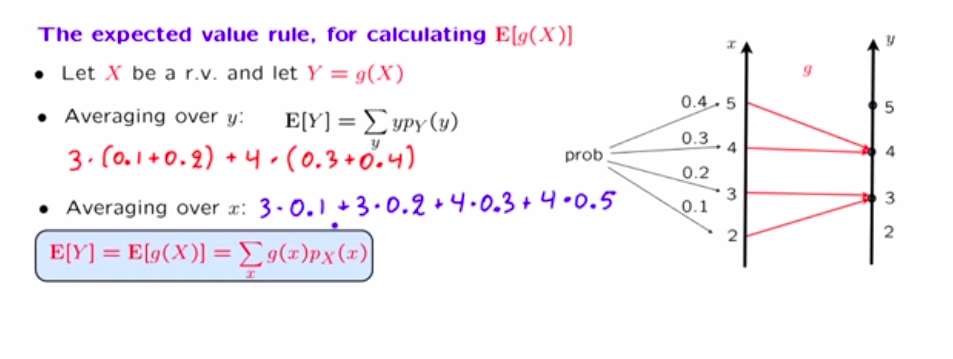
\includegraphics{img/expectedvaluerule.png}
\caption{Expected Value Rule}
\end{figure}

\begin{itemize}
\tightlist
\item
  He goes through the proof at the end of this video if you need it.
\item
  https://www.youtube.com/watch?v=gB5TCCfF6e4\&list=PLUl4u3cNGP60hI9ATjSFgLZpbNJ7myAg6\&index=59
\item
  The \emph{linearity of expectation} makes sense knowing this.
\item
  If Y is some function of x \(Y = g(x)\) and it's linear
  \(g(x) = ax + b\).
\item
  Then, \(E[g(X)] = \sum_xg(X)p_X(x)\)
\item
  \(E[g(X)] = \sum_xaxp_X(x) + \sum_xbp_X(x)\)
\item
  \(E[g(X)] = \sum_xaxp_X(x) + \sum_xbp_X(x)\)
\item
  \(E[g(X)] = aE[X] + b\)
\end{itemize}

\hypertarget{variance}{%
\subsection{Variance}\label{variance}}

\begin{itemize}
\tightlist
\item
  Expected value of the distance from the mean for random variable. Or
  just the average distance from the mean.
\item
  \(E[X - \mu]\), because this is zero, we consider the absolute value.
\item
  \(E[(X - \mu)^2] = E[X^2 -2\mu + \mu^2] = E[X^2] - E[X]\), because
  this is zero, we consider the absolute value.
\item
  \(var(aX + b) = a^2var(X)\).
\end{itemize}

\begin{center}\rule{0.5\linewidth}{\linethickness}\end{center}

\hypertarget{tips}{%
\section{Tips}\label{tips}}

\begin{itemize}
\tightlist
\item
  if you don't know the probability assign it to a variable \(p\).
\item
  Use De Morgans law for turning unions into intersections.
\item
  Think about justifying your answer intuitively.
\item
  Make assumptions really clear.
\item
  Try to calculate the outcome space and see if you can apply
  probability purely from division of this space. This uses a lot of
  counting which I'm still getting used to.

  \begin{itemize}
  \tightlist
  \item
    Event's is just a set of outcomes so can also be counted.
  \item
    Saw this in q1 problem set 3.
  \end{itemize}
\end{itemize}

\hypertarget{section}{%
\subsection{03/03/23 14:39:00}\label{section}}

\begin{itemize}
\tightlist
\item
  Can think of probability as spreading `cream cheese' in the sample
  space. If the area is the probability, a uniform distribution will
  mean all areas contain the same amount of `cream cheese'.
\end{itemize}

\hypertarget{section-1}{%
\subsection{04/03/23 17:49:00}\label{section-1}}

There's no time dimension to sets. It's encoded in the events.

\begin{itemize}
\tightlist
\item
  Finished first two problem sets (kind of).
\item
  Think I'm learning a bit about how to distribute the probability law
  over the sample space, particularly when it's non-uniform.
\item
  The Monty Hall problem is really interesting. It's counter intuitive
  and it really relies on clarifying your exact assumptions.
\item
  Using set notation can be good to remove time or spacial dimensions
  from events and add an element of flatness to your calculation. I'm
  not fully sure what I mean by this yet.
\item
  Being very careful with assumptions and building up the laws and
  sample space is important. It can be done fast by those familiar but I
  don't see anything wrong with doing it slowly for a while.
\end{itemize}

\end{document}
